\documentclass[12pt,a4paper]{article}
\usepackage[utf8]{inputenc}
\usepackage[ngerman]{babel}
\usepackage{amsmath}
\usepackage{amsfonts}
\usepackage{amssymb}

\def \blattNr{11}

	%\usepackage{xcolor}%für die Farben

\usepackage{tikz}
\usetikzlibrary{arrows,automata}

\title{Formale Grundlagen der Informatik II - Blatt \blattNr}
\author{Vincent Dahmen 6689845  \and Mirco \and Tim Jammer 6527284}




\begin{document}

\maketitle{}

\section*{\blattNr .3}
\subsection*{1.}
%\begin{align*}
B=\{
&\begin{pmatrix}
0\\0\\3\\0\\2
\end{pmatrix},
\begin{pmatrix}
0\\0\\3\\1\\1
\end{pmatrix},
\begin{pmatrix}
0\\0\\3\\2\\0
\end{pmatrix},\\
&\begin{pmatrix}
0\\5\\2\\0\\2
\end{pmatrix},
\begin{pmatrix}
0\\5\\2\\1\\1
\end{pmatrix},
\begin{pmatrix}
0\\5\\2\\2\\0
\end{pmatrix},\\
&\begin{pmatrix}
0\\10\\0\\0\\0
\end{pmatrix},
\begin{pmatrix}
8\\0\\0\\0\\0
\end{pmatrix},
\begin{pmatrix}
2\\7\\0\\0\\0
\end{pmatrix},
\begin{pmatrix}
6\\2\\0\\0\\0
\end{pmatrix}
\}
\end{align*}
Die Ersten Beiden Zeilen Beschreiben die Markierungern, bei denen c für unbeschränktheit in $p_4$ sorgt.\\
Die Letzte Zeile Beschreibt die möglichkeiten, bei denen der Zyklus a,b für unbeschränktheit z.b. in $p_3$ sorgt.


\subsection*{2.}
%\subsubsection*{a)}
Für Alle Pfade Gilt, dass wenn es einen Fehler gab solange Fehler gilt, bis nicht Batterie Gilt. Und es gilt nicht für alle Pfade das irgentwann in der Zukunft Active gilt.
\subsubsection*{b)}
Für Alle Pfade gilt In jedem Punkt, das es einen Pfad gibt, auf dem irgentwann Active gilt.
%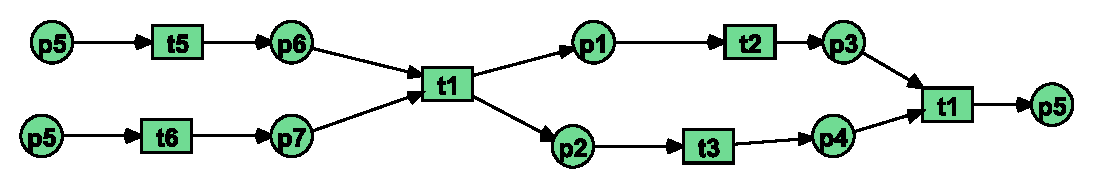
\includegraphics[scale=0.75]{Teilaufgaben/03-2.pdf}

%\subsection*{3.}
%Alle Etiketten sind $\in P(\{Locked,Battery,On,Error,Active\})$
\begin{align*}
E_S(c_0)&=\{Locked,Battery\}\\
E_S(c_1)&=\{Locked,Battery,On\}\\
E_S(c_2)&=\{Battery,On\}\\
E_S(c_3)&=\{Battery,On,Active\}\\
E_S(c_4)&=\{Locked,Battery,Error\}\\
E_S(c_5)&=\{Locked\}
\end{align*}
es ergibt sich (durch einfaches austauschen der Zustände durch ihre entsprechenden ettiketten):
\begin{align*}
 E_S(SS(M_{cell}))=&( \{Locked,Battery\}\{Locked,Battery,On\}\\
 &(\{Battery,On\}\{Locked,Battery,On\})^*\\
 &(\{Battery,On,Active\}\{Battery,On,Active\}^*\{Battery,On\})^*\\
 &(\{Locked,Battery\} + \\
 &(\{Battery,On,Active\}\{Battery,On,Active\}^*\\
 &\{Locked,Battery,Error\}\{Locked,Battery,Error\}^*\\
 &\{Locked\}\{Locked,Battery\})))^\omega
 \end{align*}

%\subsection*{4.}
%Ja, da $c_0\in Sat(f)$ gilt.

%\subsection*{5.}
%Nein, die Formel glt nicht.
Beispielsweise die rechnung
\[c_0c_1c_2c_3c_4c_5(c_0c_1c_2)^\omega\]
erfüllt die Formel nicht. in $c_4$ gilt Error, allerdings gilt danach nie wieder Active
%
%\subsection*{6.}
%Wir setzen das Kantengewicht der kante von $p_2$ nach $t_4$ auf 1\\
\begin{tikzpicture}[->,>=stealth',shorten >=1pt,auto,node distance=2.8cm,
                    semithick]
  \tikzstyle{every state}=[fill=none,draw=none,text=black]

  \node[state] (020)            				{$\begin{pmatrix} 0 \\2\\0 \end{pmatrix}$};
  \node[state] (110) [ above of=020]    		{$\begin{pmatrix} 1 \\1\\0 \end{pmatrix}$};  
  \node[state] (200) [ right of=110]         	{$\begin{pmatrix} 2 \\0\\0 \end{pmatrix}$};
  \node[state] (101) [ left of=020]        	{$\begin{pmatrix} 1 \\0\\1 \end{pmatrix}$};  
  \node[state] (011) [ below of=020]           	{$\begin{pmatrix} 0 \\1\\1 \end{pmatrix}$};
  \node[state] (002) [ right of=011]  		   	{$\begin{pmatrix} 0 \\0\\2 \end{pmatrix}$};
   

 

  \path (110) edge [bend left]         node {$t_2$} (200)
 		(110) edge [bend left]         node {$t_1$} (020)
 		(110) edge          node {$t_4$} (101)
		
 		(200) edge [bend left]         node {$t_1$} (110)

		(101) edge          node {$t_1$} (011)
		(101) edge [bend left]         node {$t_3$} (110)
 		
		(020) edge         node {$t_2$} (110)
 		(020) edge [bend left]         node {$t_4$} (011)
 		
		(011) edge [bend left]         node {$t_2$} (101)
		(011) edge         node {$t_3$} (020)
		(011) edge [bend left]         node {$t_4$} (002) 
		
		(002) edge [bend left]         node {$t_3$} (011)		
	
		;
        

\end{tikzpicture}



\pagebreak

\section*{\blattNr .4}

\subsection*{1.}

%Alle Transtionssysteme sind Bisimilar:
\[TS_1 \underline{\leftrightarrow} TS_2: \mathcal{B}=\{(q_0,r_0),(q_1,r_1),...\}=\{(q_0,r_i)|i\  mod\  2 =0)\}\cup \{(q_1,r_i)|i\  mod\  2 \not = 0 \}\} \]

\[TS_1 \underline{\leftrightarrow} TS_3: \mathcal{B}=\{
(q_0,s_0),(q_1,s_1),(q_0,s_2),(q_1,s_3)\} \]

\[TS_2 \underline{\leftrightarrow} TS_3: \mathcal{B}=\{(r_0,s_0),(r_1,s_1)\}\cup \{(r_i,s_2)|i\  mod\  2 =0,\ i\geq 2)\}\cup \{(r_i,s_3)|i\  mod\  2 \not = 0,\ i\geq 3 \}\} \]

%
\subsection*{2.}
%%\includegraphics[scale=0.5]{Teilaufgaben/Aufgabe2.pdf}
%\begin{align*}
t_6&=(\underline{(b+b+b)}(\underline{(c+c)}+a) (c\underline{(d+d)}+\underline{(c+c)}\cdot \underline{(d+d)})\\
&=b(c+a) \underline{(cd+cd)}\\
&=b(c+a)cd\\
&=b(\underline{(c+a)cd)}\\
&=b(ccd +acd)\\
\end{align*}

$t_5$ und $t_6$ sind nicht äquivalent, da die normalformen unterschiedlich sind.


Um Die Benötigte Funktionalität zu Modellieren benötigt man nur einen Platz und 3 Transtitonen:\\
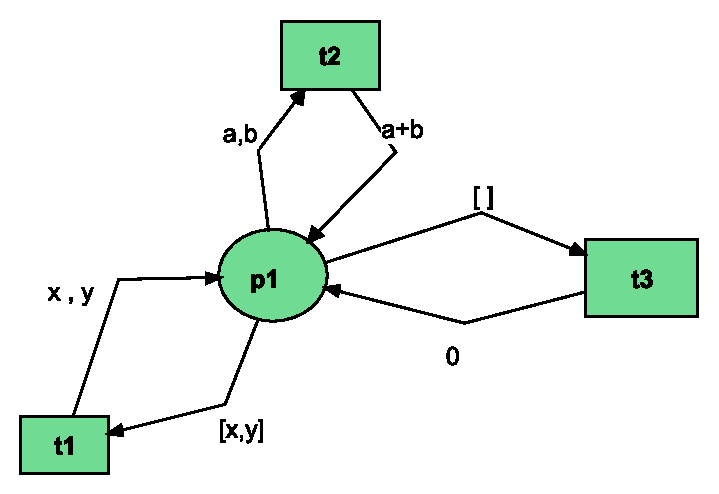
\includegraphics[scale=1.0]{Teilaufgaben/einfach.pdf}\\
Startmarkierung in $p_1$ muss der Baum sein, das Netz Verklemmt genau dann wenn das Ergebnis in $p_1$ als markierung liegt.\\
$t_1$ baut dabei den Baum Auseinander, $t_2$ addiert alle Zahlen, die dabei in $p_1$ hineingelegt werden. $t_3$ dekt den Sonderfall des Leeren Baums ab.\\
\\
Die Markerung x , y bezeichnet, das die elemente x und y an die Stelle $p_1$ gelegt werden.
\\
Übertragen in die Benötigte Form mit anfangs und endtransition benötigt man noch einen Zähler, der Die Anzahl an additionen (= die Anzahl an Knoten im Baum, die Keine Blätter sind) mitzählt, um zu wissen, wann das ergebnis Fertig berechnet ist, da die Letzte Transition nur dann schalten darf.
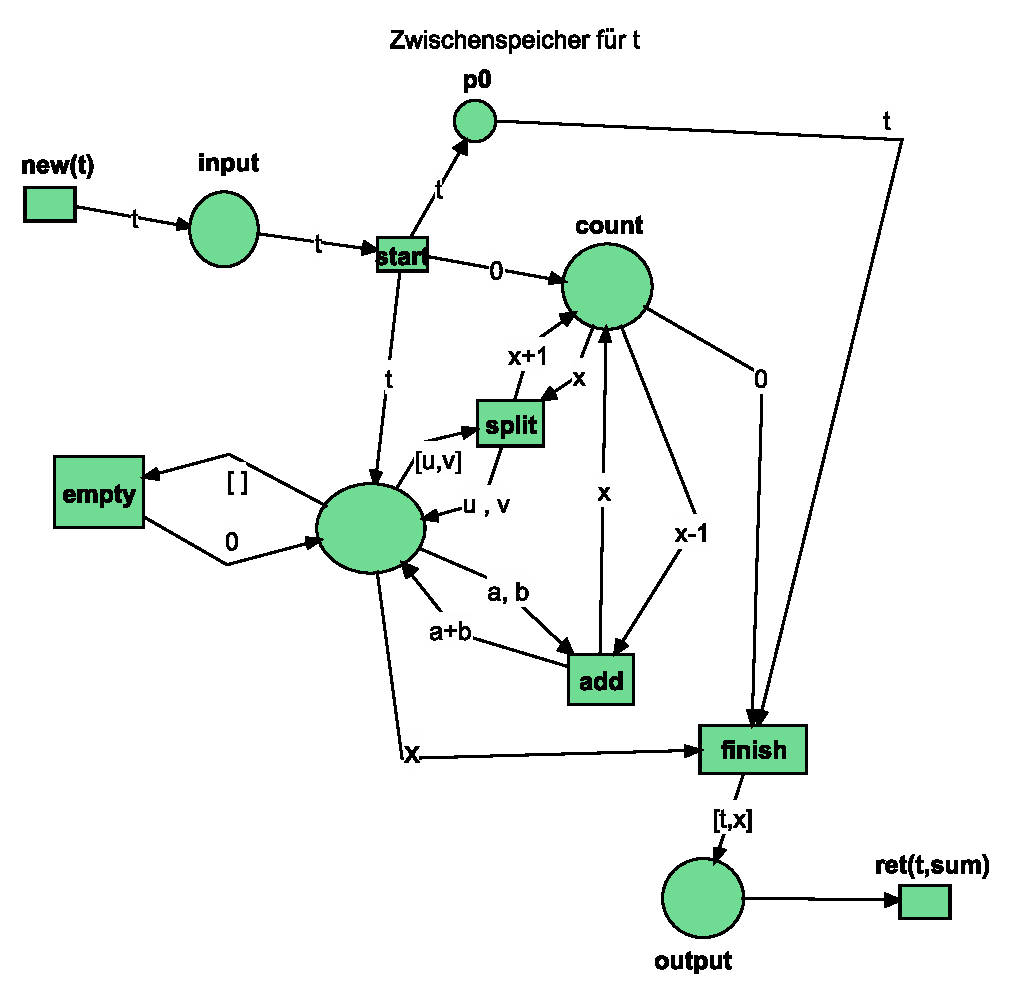
\includegraphics[scale=0.8]{Teilaufgaben/erweitert.pdf}
%%
%\subsection*{3.}
%\[(r+e+d)^*\cdot r\cdot e\cdot d\cdot(r+e+d)^*\]
auf die Klammern wurde, wo möglich, verzichtet
%%\includegraphics[scale=0.5]{Teilaufgaben/Aufgabe3.pdf}
%
%\subsection*{4.}
%
\begin{tikzpicture}[->,>=stealth',shorten >=1pt,auto,node distance=2.8cm,
                    semithick]
  \tikzstyle{every state}=[fill=none,draw=black,text=black]

     \node[initial, state,accepting] (b1)[ below of=r1gr2]    {$B_1$};

  \node[state] (b2)   [ right of=b1]     {$B_2$}; 
     
  
   \node[state] (b3) [ right of=b2]	{$B_3$};  
     
 
    \node[state] (b4) [ right of=b3]	{$B_4$};
 
     
     
 
  \path   
  	  (b1) edge 	node {$rg_1,g_2$}	(b2)   	  
    
 	  (b2) edge 	node {$gr_1,r_2$} (b3)    
  	  
  	   	  (b3) edge 	node {$g_1,rg_2$}	(b4)    	  
  	  
  	  (b4) edge [bend left] node  {$r_1,gr_2$}	(b1)
  
  	
		;
        

\end{tikzpicture}
%%\includegraphics[scale=0.5]{Teilaufgaben/Aufgabe4.pdf}
%
%\subsection*{5.}
%%\includegraphics[scale=0.5]{Teilaufgaben/Aufgabe5.pdf}
%
\begin{tikzpicture}[->,>=stealth',shorten >=1pt,auto,node distance=2.8cm,
                    semithick]
  \tikzstyle{every state}=[fill=none,draw=black,text=black]

     \node[initial, state] (b1m1)   {$B_1M_1$};

  \node[state] (b2m1)   [ right of=b1m1]     {$B_2M_1$}; 
     
  
   \node[state] (b3m1) [ right of=b2m1]	{$B_3M_1$};  
     
 
    \node[state] (b4m1) [ right of=b3m1]	{$B_4M_1$};
    
  \node[state,accepting] (b1m2)[ below of=b1m1]    {$B_1M_2$};

  \node[state] (b2m2)   [ right of=b1m2]     {$B_2M_2$}; 
     
  
   \node[state] (b3m2) [ right of=b2m2]	{$B_3M_2$};  
     
 
    \node[state] (b4m2) [ right of=b3m2]	{$B_4M_2$};
 
     
     
 
  \path   
  	  (b1m1) edge 	node {$rg_1,g_2$}	(b2m1)   	  
    
 	  (b2m1) edge 	node {$gr_1,r_2$} (b3m1)    
  	  
  	   	  (b3m1) edge 	node {$g_1,rg_2$}	(b4m1)    	  
  	  
  	  (b4m1) edge [bend left] node  {$r_1,gr_2$}	(b1m1)
  	  
  	  
  	  
  	    	  (b1m2) edge 	node {$rg_1,g_2$}	(b2m2)   	  
    
 	  (b2m2) edge 	node {$gr_1,r_2$} (b3m2)    
  	  
  	   	  (b3m2) edge 	node {$g_1,rg_2$}	(b4m2)    	  
  	  
  	  (b4m2) edge [bend left] node  {$r_1,gr_2$}	(b1m2)
  
  	
		;
        

\end{tikzpicture}
%%
%\subsection*{8.}
%\includegraphics[scale=0.5]{Teilaufgaben/Aufgabe6.pdf}
%Angenommen das Netz Sei Vor dem Anwenden Der regel Beschränkt, so ist dies Auch nach dem Anwenden Der Regel der Fall, Das Entfernen einer Transition, kann die Beschränktheit nicht zerstören.\\
Angenommen das Netz sie Vor dem anwenden Der Regel unbeschränkt, so ist es dies auch nach dem Anwenden Der Regel, Da Jedes Auftreten von der Entfernten Transition in irgenteiner Schaltfolge durch die Weiterhin vorhandene Transition mit gleihcem vor und Nachbereich ersetzt werden kann, ohne die Auftretenden Markierungen zu ändern.

\end{document}
